\section{Controlled Geometry Reference Model (G-054--G-057)}
\label{sec:phase-diagram}

The G-track is a series of controlled NumPy toy experiments that demonstrate accessible
mechanisms in engineered geometry --- where embedding roles, head functions, and parameter
sweeps are exactly specified.
The architecture across G-055--G-057 is a 6-layer transformer (NumPy only, no training;
$D=16$; 8 geometric dims + 8 FIN dims; variable SEED).
G-054 uses a 12-layer BERT variant with semantic Q/K/V initialization.
The G-track is not a calibrated predictor of T5-small behavior; it is a reference model
for structural phenomena that are difficult to isolate in a trained system.
The relationship between G-track findings and S-track findings is analogy and structural
convergence, not quantitative prediction.

\subsection{Three Regimes: Slow-Collapse, Sharp-Collapse, No-Collapse (G-054)}

G-054 sweeps the bank token's FIN embedding weight
(\texttt{FIN\_WEIGHT} $\in \{0.0, 0.1, 0.2, 0.3, 0.5, 0.7, 1.0, 1.5, 2.0\}$) in a
12-layer BERT (semantic Q/K/V init, SEED=54) and measures the per-head Born filter
H1(FIN) ratio at every layer.
Three regimes emerge:

\begin{itemize}
  \item \textbf{Slow-collapse} (\texttt{FIN\_WEIGHT} $\leq 0.1$): the FIN specialist
    head collapses in S3 gradually over many layers.
    Peak ratio occurs at a late layer (layer 11), magnitude approximately $2\times$.
    This is a modest late-layer amplification.

  \item \textbf{Sharp-collapse} (\texttt{FIN\_WEIGHT} $= 0.1$--$0.3$): the FIN
    specialist head collapses at a specific mid-layer in a single step.
    At \texttt{FIN\_WEIGHT}$=0.3$, the S3 H1 defect drops from $1.268$ at layer~5
    to $0.012$ at layer~6 --- a near-zero denominator with a finite numerator.
    The Born filter ratio reaches $8.79\times$ at layer~5 and $867\times$ at layer~6.
    This is the super-amplification zone.

  \item \textbf{No-collapse} (\texttt{FIN\_WEIGHT} $\geq 0.5$): the bank token carries
    sufficient FIN signal that the FIN specialist head finds genuine FIN content to
    attend to in S3; no collapse occurs.
    Ratio peaks at layer~1 and decays monotonically through later layers (ratio $< 1\times$
    at the specialist layers).
\end{itemize}

The phase transition between sharp-collapse and no-collapse is confirmed sharp, occurring
between \texttt{FIN\_WEIGHT}$=0.3$ and \texttt{FIN\_WEIGHT}$=0.5$
(H2 confirmed; H1 near-miss: \texttt{FIN\_WEIGHT}$=0.0$ ratio $= 1.9976\times$,
missed $2.0\times$ threshold by $0.0024$).
The collapse speed --- how quickly the FIN head reaches self-attention in S3 ---
determines both the peak layer and the peak ratio.

Figure~\ref{fig:phase-diagram} shows the three-regime structure.

\begin{figure}[t]
\centering
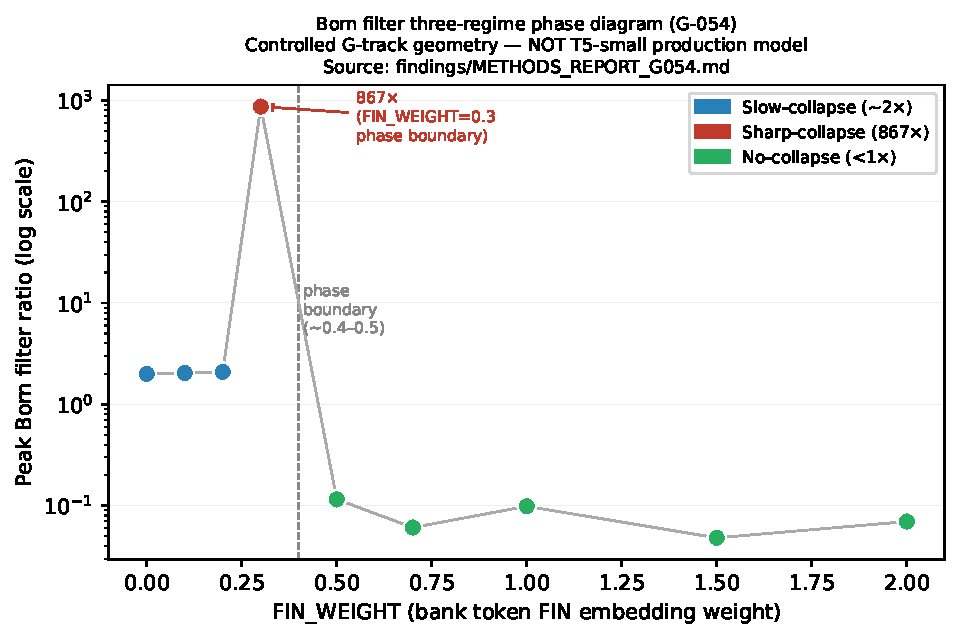
\includegraphics[width=0.82\linewidth]{figures/fig05_three_regime_phase_diagram}
\caption{Born filter three-regime phase diagram (G-054). Controlled NumPy G-track
geometry --- \emph{not} the T5-small production model.
\texttt{FIN\_WEIGHT} sweeps the bank token's FIN embedding component.
Three regimes: slow-collapse (${{\approx}}2\times$), sharp-collapse
($867\times$ at \texttt{FIN\_WEIGHT}=0.3), no-collapse ($<1\times$).
Phase transition at \texttt{FIN\_WEIGHT}~$\approx 0.4$--$0.5$.
Source: \texttt{METHODS\_REPORT\_G054.md}.}
\label{fig:phase-diagram}
\end{figure}

\subsection{Super-Amplification at the Phase Boundary}

The $867\times$ peak at \texttt{FIN\_WEIGHT}$=0.3$ is the ratio of two quantities that
nearly cancel: at layer~6 the S3 H1 defect drops to $0.012$ while the S1 numerator
remains finite, so the ratio diverges.
This is not a qualitative peak --- it is a structural divergence at a near-cancellation
point.
The same structural property appears in the production near-cancellation result (S-059b):
cross-attention $-171.25$ and FFN correction $+165.25$ nearly cancel to a residual of
$-6.005$ (\S\ref{sec:explaining}).
These two amplification values are not the same metric:
the G-track $867\times$ is a Born-filter H1 ratio (S\_success/S\_fail at specialist layers);
the S-track $28.52\times$ is the ratio between the cross-attention partial margin and the
observed final logit margin.
The analogy is denominator-small amplification under near-cancellation, not identity
of measurement.
The two systems are not calibrated to each other; both independently exhibit the
near-cancellation structure where a small residual is the difference of two large opposing
terms, and the signal diverges near the cancellation point.

The phase boundary defines where Born filter measurement is most informative:
in the sharp-collapse regime, a small change in the bank token's FIN content can produce
an order-of-magnitude change in the Born filter ratio.
The slow-collapse and no-collapse regimes produce bounded, modest signals.

\subsection{Head Causal and Diagnostic Distinction (G-055, G-056)}

G-054 maps the parameter landscape; G-055 and G-056 test which head types are causally
load-bearing versus diagnostic within that landscape.

\paragraph{Global-engagement head as diagnostic (G-055).}
G-055 places a global head (Q/K = $0.005 \times \mathbf{1}$, producing near-uniform
attention; V $= I$) at layer~3 of a 6-layer NumPy toy.
S\_success uses \texttt{FIN\_WEIGHT}$=0.5$ (no-collapse regime); S\_fail uses
\texttt{FIN\_WEIGHT}$=0.05$ (slow-collapse regime).
Ablating the global head changes the specialist-layer Born filter ratio by $4\%$
($1.87\times \to 1.94\times$).
The layer-2 near-identity control ablation produces the same $4\%$ change.
Pearson $r(\text{L3 defect},\ \text{L5 defect})$ is $+1.0000$ before ablation and
$+0.9999$ after, confirming that layer~3 and layer~5 both track the same underlying
quantity --- the bank token's FIN content in the residual --- in parallel, not via
mediation.
Conclusion: the global-engagement head is diagnostic.
Its Born filter ratio reflects the upstream embedding difference it observes; removing it
does not change what the downstream specialist heads see.

\paragraph{Suppressive head: diagnostic below, causal above FIN-annihilation (G-056).}
G-056 replaces the global head's value matrix with
$W_V = I - \alpha \cdot P_\text{FIN}$ and sweeps $\alpha \in \{0.0, 0.5, 1.0, 1.5, 2.0\}$.

\begin{itemize}
  \item $\alpha=0$: neutral head (G-055 reference). Ablation change: $1.2\%$. Diagnostic.
  \item $\alpha=0.5$: partial FIN suppression. Ablation change: $1.0\%$. Diagnostic.
  \item $\alpha=1.0$: FIN-annihilation (maps FIN component to zero). Ablation change:
    \textbf{exactly $0\%$}. The head has no causal effect when it reduces FIN content
    to zero without inverting it.
  \item $\alpha=1.5$: FIN-inversion begins. Ablation change: $6.7\%$.
  \item $\alpha=2.0$: FIN fully inverted. Ablation change: \textbf{$42\%$}
    ($5.06\times$ baseline $\to 2.93\times$ ablated). Layer-1 control: $0.1\%$.
\end{itemize}

The causal mechanism is not signal removal but re-routing.
At $\alpha=2.0$, the suppressive head inverts the bank token's FIN content (residual FIN
at bank: $1.708 \to 0.051$ for S\_success, $1.114 \to 0.306$ for S\_fail).
After inversion, S\_fail bank carries more FIN content than S\_success bank --- the
success/fail ordering is reversed.
FIN-specialist heads then re-route attention toward bank (attention to bank: $0.013$
when head is ablated $\to 0.168$ when head is active) and amplify the inverted signal.
The $42\%$ ablation change reflects the removal of this re-routing, not the restoration
of a blocked signal.
In short, the inverted head changes what the specialist heads treat as FIN-bearing
evidence; ablation removes that induced re-routing rather than merely restoring a
suppressed signal.

The G-054 connection: the suppressive head at $\alpha=2.0$ performs a regime shift
on the downstream computation, pushing S\_success bank from the no-collapse regime
(\texttt{FIN\_WEIGHT}$\approx 0.5$) toward the slow-collapse regime (\texttt{FIN\_WEIGHT}
near zero).
A neutral or mildly suppressive head ($\alpha < 1.0$) does not shift regimes and
remains diagnostic.

\subsection{Near-Cancellation and Inversion at Toy Scale (G-057)}

G-057 extends G-056 by introducing an FFN correction parameter $\gamma$ that partially
cancels the global head's FIN contribution
($\mathrm{FFN}(h) = h - \gamma \cdot P_\text{FIN} \cdot \mathrm{head\_output}$)
and sweeps $\gamma$ from 0 to 2.
At $\gamma=1.0$ (exact FIN cancellation by the FFN), the Born filter reconstruction
fraction diverges to $\infty$ ($9{,}184\times$ measured), mirroring the production
near-cancellation structure from S-059b.
At $\gamma=2.0$ (FFN over-correction), G-057 reproduces the G-056 FIN-inversion:
$51.3\%$ ablation change at specialist layers.
G-057 also shows the directional sign-reversal analog to S-060: ablating the corrective
FFN component worsens Born filter discrimination, while ablating the upstream source
improves it.

The detailed near-cancellation account, including the two-track convergence figure
(Fig.~\ref{fig:two-track}), is in \S\ref{sec:explaining}.
G-057's role here is to provide controlled evidence that the near-cancellation structure
is not specific to the G-057 model parameters or to the S-059b measurement protocol:
the same structural divergence appears independently in both controlled geometry and in
the production system.

\subsection{What This Does Not Establish}

\begin{itemize}
  \item \textbf{Which regime T5-small occupies.}
    G-054 maps three regimes by the bank token's FIN embedding weight.
    Whether T5-small's OOD jump encoder representation places the decoder in the
    slow-collapse, sharp-collapse, or no-collapse regime requires direct per-layer
    Born filter profiling on the production model.
    The $28.52\times$ reconstruction fraction (S-059b) is consistent with a near-cancellation
    point in the sharp-collapse regime, but the correspondence is structural, not calibrated.

  \item \textbf{The causal regime of L3H4 in T5-small.}
    G-056 identifies a threshold at the FIN-annihilation point ($\alpha=1.0$).
    L3H4's mild suppressive cosines ($\cos_\text{walk,fail}=-0.044$,
    $\cos_\text{jump,fail}=-0.026$) are at most suggestive of diagnostic-like behavior;
    they do not classify the production head's regime.
    G-056 supplies the controlled threshold concept ($\alpha=1.0$ annihilation boundary),
    not a regime assignment for L3H4.
    L3H4 is neither confirmed causal nor confirmed diagnostic by the G-track experiments.

  \item \textbf{Quantitative correspondence between G-track and S-track values.}
    The G-track uses engineered embeddings, fixed seeds, and NumPy-only computation.
    Its Born filter ratios, $\alpha$ thresholds, and $\gamma$ sweep values are not
    calibrated to T5-small's logit magnitudes, head norms, or training distribution.
    The $867\times$ peak (G-054) and the $9{,}184\times$ measured divergence (G-057)
    demonstrate structural phenomena; they are not predictions of T5-small's amplification
    magnitude.

  \item \textbf{Generalization to other trained architectures.}
    G-track results are established in controlled NumPy geometry.
    Whether the three-regime structure, the FIN-annihilation threshold, and the
    near-cancellation divergence appear in transformers with learned weights,
    layer normalization, and full training distributions is an open question.
    The S-track evidence is the direct source for production claims.
\end{itemize}
